Since the $0\nu\beta\beta$ decay of $^{76}$Ge has a $Q$-value of 2.039~MeV, natural $\gamma$-rays with energies larger than 2.039~MeV are the main background sources for GERDA. Fortunately, the spacial distribution of photon induced signals in a germanium detector is quite different from that of electron induced signals due to their different interactions with germanium as described in Sec.~\ref{sec:det:phys}. Segmented germanium detectors will be used in GERDA Phase II in order to identify photon induced background. The discrimination power of segmented germanium detector for photon induced background were examined systematically\cite{Pid07} using GERDA Phase II prototype detector Siegfried I (see Sec.~\ref{sec:gerda:stat3}) and its test stand (see Sec.~\ref{sec:tt:comc}). The main results are summarized in this chapter. 

MaGe~\cite{Mag08}, a C++ simulation package is co-developed by the Majorana and GERDA collaborations based on Geant4 toolkits~\cite{Gea03,Gea06}. It was used for the simulation of GERDA and the detector test facilities in Munich. The simulation of photon induced events was proved to be better than 5\%.

\section{Event classification}
\label{sec:ph:eve}
As described in Sec.~\ref{sec:det:gamma} a photon with an energy of the order of one MeV has a mean free path of several centimeters in the germanium crystal. It most probably deposits energy in several different places and create \emph{multi-site event}. On the other hand, the average range of a 1~MeV electron in germanium is about 0.5~mm (see Sec.~\ref{sec:det:ep}). Since the spacial resolution of germanium detectors is larger than 1~mm\footnote{Preliminary simulation carried out recently by Majorana collaboration indicates the point contact detector may have spacial resolution better than 1~mm with pulse shape analysis.}, electrons mainly create \emph{single-site events}. Segmented germanium detectors can be used to distinguish photon-like and electron-like events based on this feature. If there is only one segment with an energy deposition, it is called a \emph{single-segment event}. In contrast, if there are more than one segment with energy depositions, it is called a \emph{multi-segment event}. 

Figure~\ref{fig:ph:eve} depicts the definitions of these four types of events and possible combinations of them. Most photon induced background events are multi-site and multi-segment events, as shown in the bottom right corner of Fig.~\ref{fig:ph:eve}. Most electron induced events are single-site and single-segment events, as shown in the top left corner of Fig.~\ref{fig:ph:eve}. By requiring anti-coincidence most of the photon induced background events can be rejected. However, there are still some photon induced multi-site events with energy deposition only in one segment, as shown in bottom left corner of Fig.~\ref{fig:ph:eve}. This kind of events can be further identified using pulse shape analysis. A single-site event can also be a multi-segment event if it happens to occur on the boundary of two neighboring segments and induces signals in both segments, as shown in the top right corner of Fig.~\ref{fig:ph:eve}. This kind of events will be rejected erroneously by the anti-coincidence requirement, and should be identified using pulse shape analysis.

\begin{SCfigure}[][htbp]
\centering
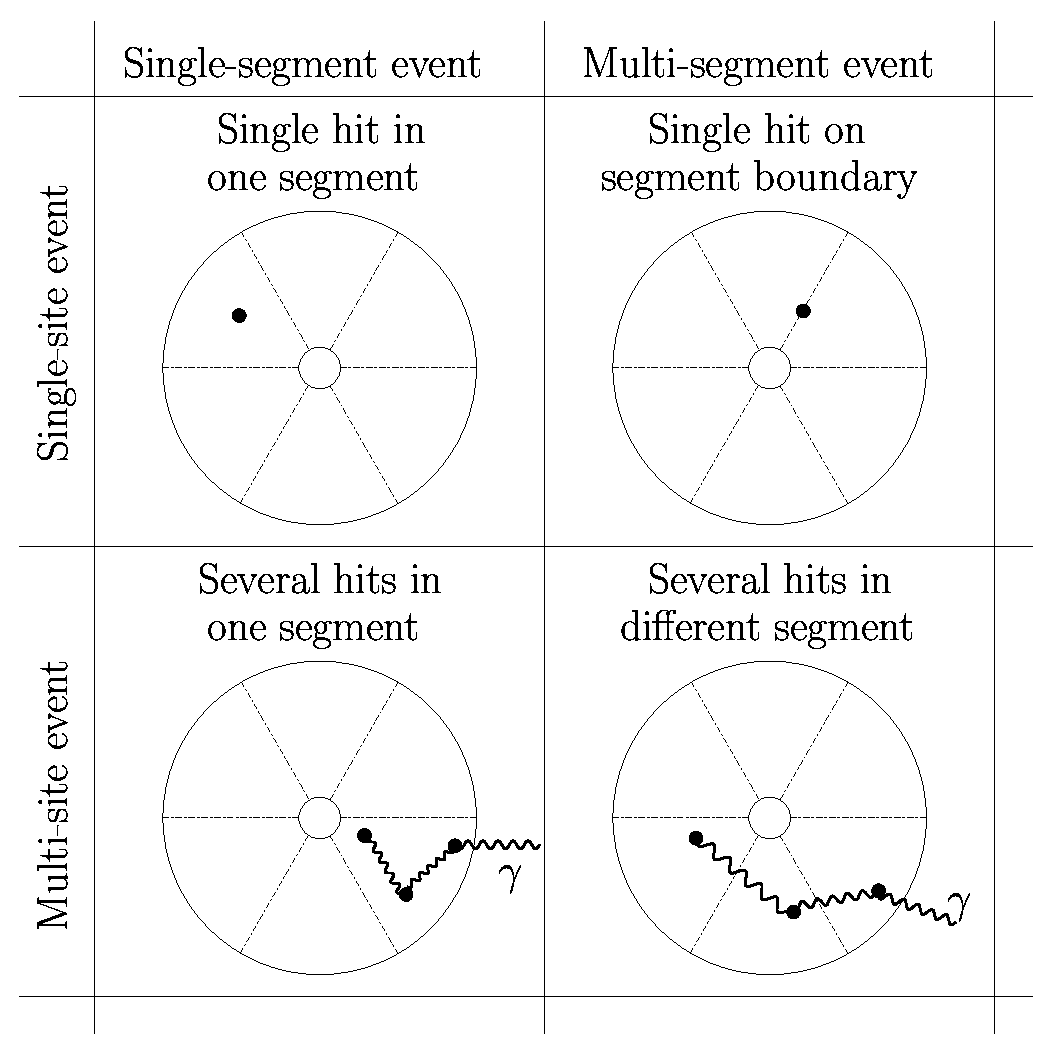
\includegraphics[width=0.5\textwidth]{events}
\caption{Event classification. The four pairs of concentric circles indicate the cross sections of Siegfried-like detectors. The dashed lines indicate the segmentation scheme. The black dots are hits (energy depositions). The wave lines indicate $\gamma$-rays.}
\label{fig:ph:eve}
\end{SCfigure}

\section{Background rejection using segmentation}
\label{sec:ph:seg}
Different data samples were taken using segmented germanium detector Siegfried I (see Sec.~\ref{sec:gerda:stat3}) and its test stand (see Sec.~\ref{sec:tt:comc}) with $^{228}$Th or $^{60}$Co $\gamma$ sources placed 10~cm above the vacuum can (see Fig.~\ref{fig:tt:comcryo}). Figure~\ref{fig:ph:seg} taken from Ref.\cite{Pid07} shows the core energy spectrum of the $^{228}$Th data sample for all events (black) and single-segment events (grey). The double escape peak (DEP in short) from $^{208}$Tl ($1\,593$~keV) is hardly suppressed while the $^{212}$Bi line ($1\,620$~keV) is suppressed by a factor of $2.85 \pm 0.01$. Since the DEP events by definition are single-segment events, Fig.~\ref{fig:ph:seg} shows clearly that photon induced events are mostly multi-segment events and can be rejected using segment anti-coincidence requirement.

\begin{figure}[htbp]
\centering
\subfloat[Core spectrum up to 3~MeV]{\label{fig:ph:sega}
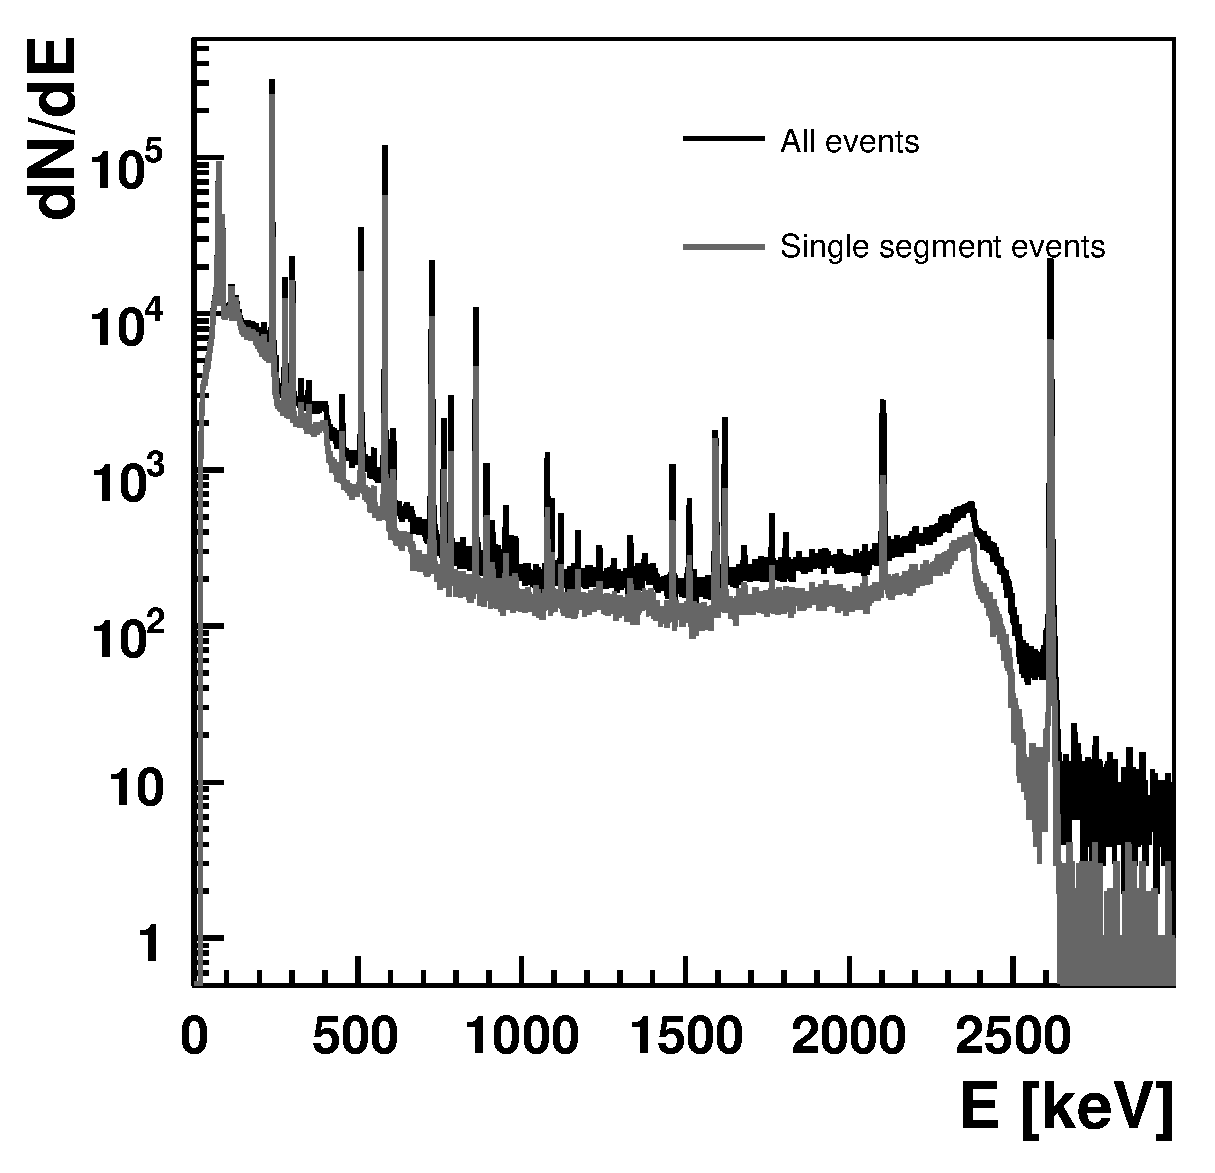
\includegraphics[width=0.4\textwidth]{energy_th228_suppression_all}}%
\subfloat[Core spectrum around 1.6~MeV]{\label{fig:ph:segb}
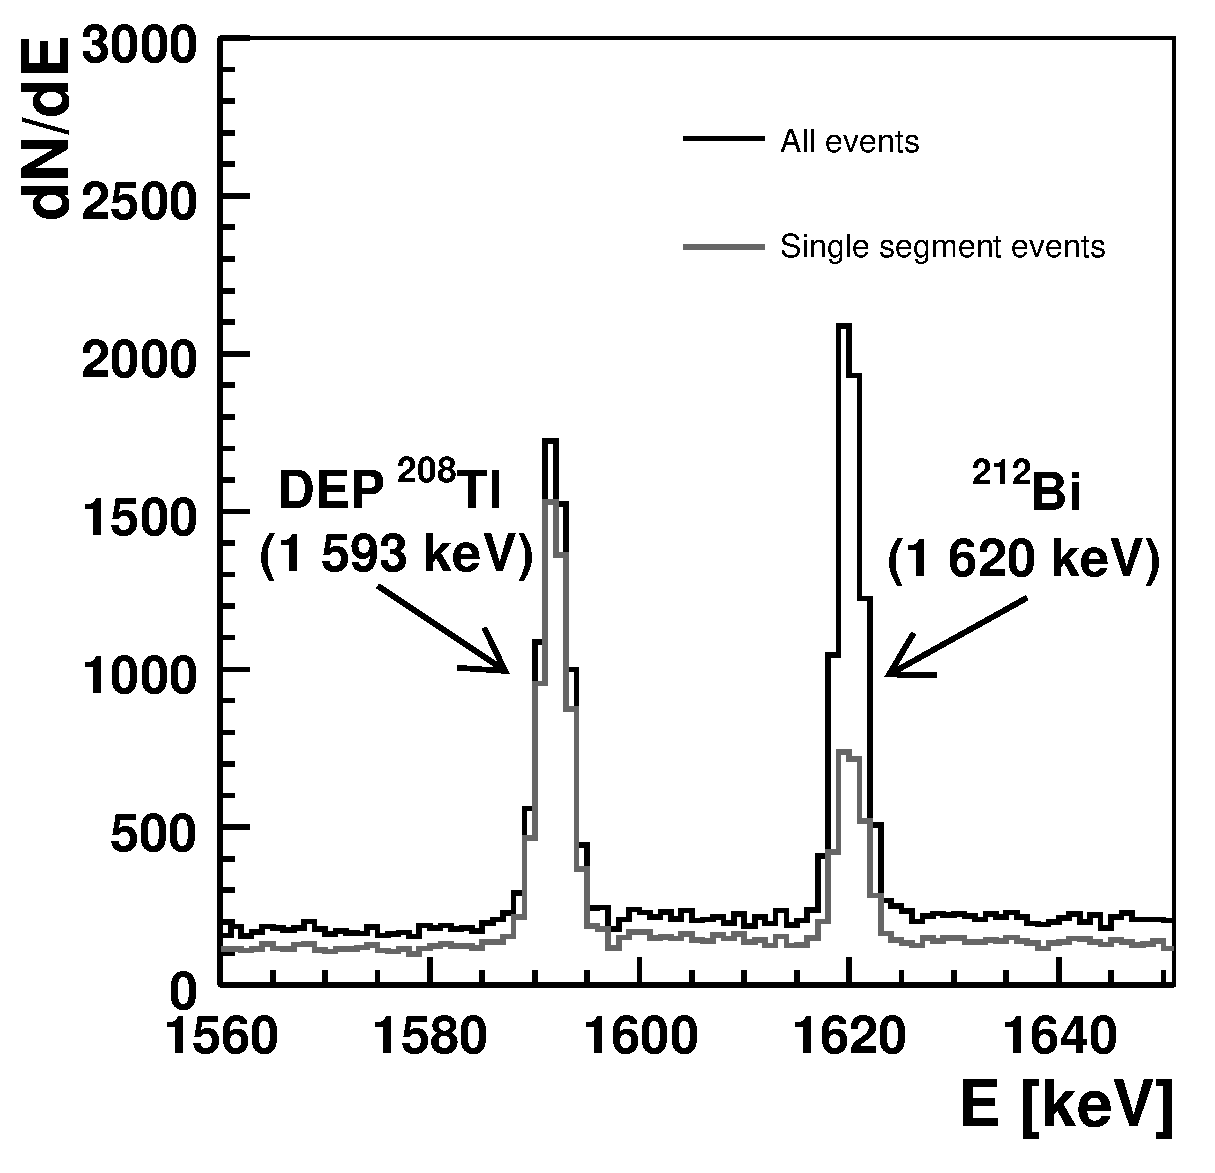
\includegraphics[width=0.4\textwidth]{energy_th228_suppression_ROI}}%
\caption{Core energy spectrum of the $^{228}$Th source data sample for all events (black) and single-segment events (grey). The double escape peak from $^{208}$Tl ($1\,593$~keV) is hardly suppressed while the $^{212}$Bi line ($1\,620$~keV) is suppressed by a factor of $2.85 \pm 0.01$.}
\label{fig:ph:seg}
\end{figure}

\section{Monte Carlo simulation}
\label{sec:ph:sim}
Monte Carlo (MC) simulations of prototype detectors and their cryostats was performed using MaGe~\cite{Mag08}, a C++ package co-developed by the Majorana and GERDA collaborations using Geant4 toolkits~\cite{Gea03,Gea06}. Figure~\ref{fig:ph:sim} shows the geometry models of the detectors and cryostats implemented in Geant4.
Figure~\ref{fig:ph:s2} shows a close-up of the \emph{Siegfried} II geometry. It was modeled in such a way that the details were implemented as close as possible to reality while the simulation efficiency did not decrease too much.

\begin{figure}[tbhp]
\centering
\subfloat[Siegfried I and its cryostat]{\label{fig:ph:s1}
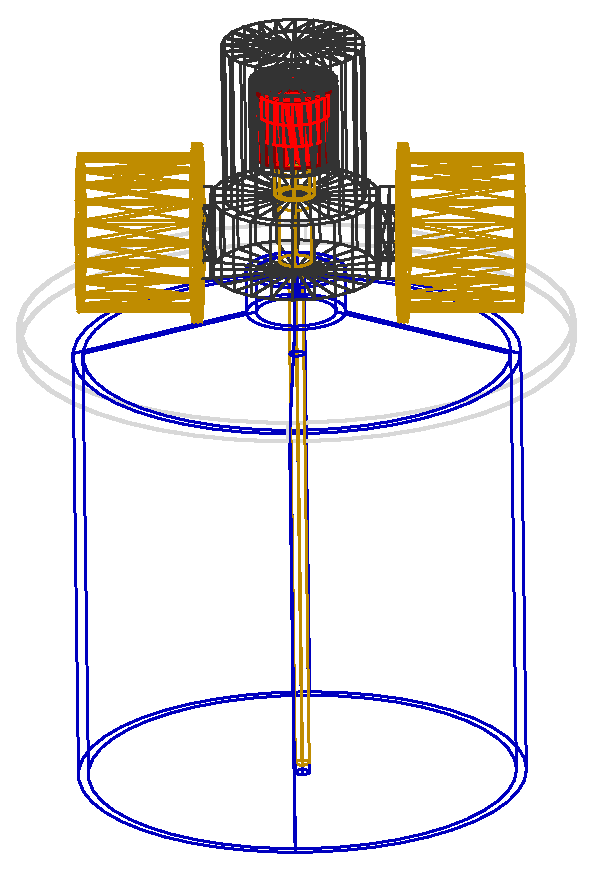
\includegraphics[height=0.3\textheight,clip]{SIwired}}
\subfloat[Gerdalinchen II]{\label{fig:ph:g2}
  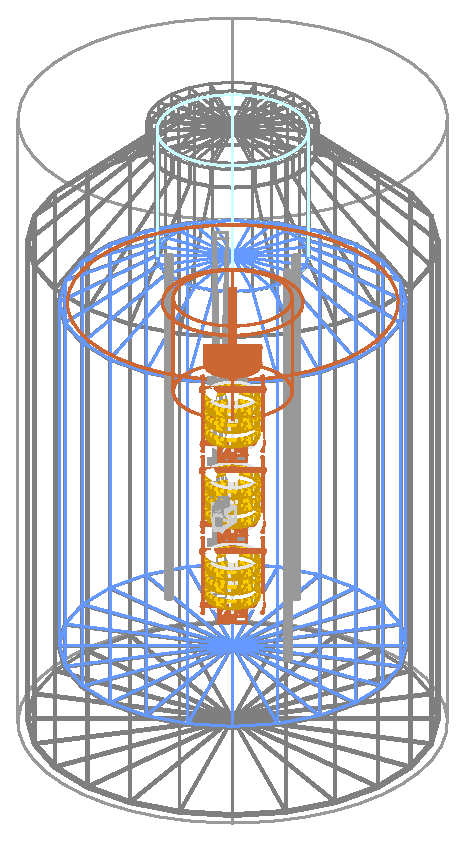
\includegraphics[height=0.3\textheight,clip]{GIIwired}}
\subfloat[Siegfried II and its frame in GII]{\label{fig:ph:s2}
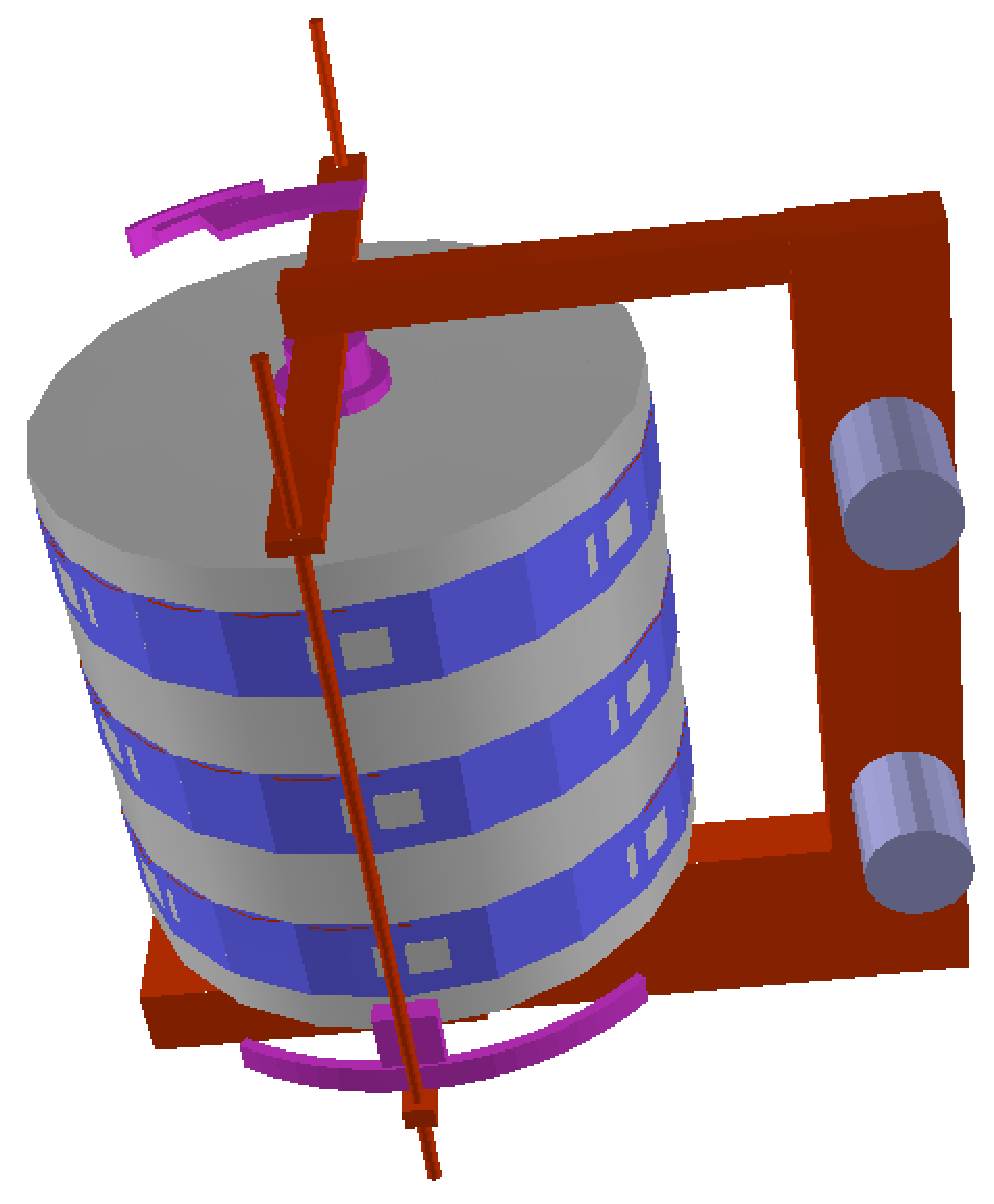
\includegraphics[height=0.3\textheight,clip]{SIIsolid}}
\caption{Detectors and their test stands geometry models in Geant4: (a) wired drawing of Siegfried I and its cryostat, (b) wired drawing of GII, and (c) a close-up of Siegfried II geometry with copper frame as used in GII.}
\label{fig:ph:sim}
\end{figure}

The energy depositions of hits in each segment were recorded and the core energy was calculated by adding all segment energies. The segment and core energies were individually smeared according to the energy resolutions of the detectors measured in the individual channels.

The spacial and time information of hits were also recorded, which served as parts of the input for the pulse shape simulation package. The geometry of detectors and the voltage bias applied were other input information for the pulse shape simulation. The detail of the pulse shape simulation is described in Chapter~\ref{cha:pss}.
 

\section{Verification of simulation}
\label{sec:ph:var}
The simulation of photon interactions with the segmented germanium detector was verified for several quantities under study: (a) the energy spectrum, (b) the occupancy of each segment, namely, the number of events recorded by each segment (see Fig.~\ref{fig:ph:occ} for measurement setup), (c) the multiplicity, namely, the number of segments having signals, and (d) the line suppression factor (SF$_{\text{L}}$) defined as the ratio of the number of total events over the number of single-segment events within the energy window $[E_{\gamma} - 3\sigma, E_{\gamma} + 3\sigma]$ where $E_{\gamma}$ is the central energy of the gamma line and $\sigma$ is the energy resolution of the line.\footnote{The suppression factors were calculated after the background was subtracted.} The simulated distributions of (a), (b) and (c) were added to the background distribution measured, and then compared to the data as shwon in the (a), (b) and (c) plots of Fig.~\ref{fig:ph:mc}. The line suppression factors were calculated for data and MC, respectively, and then compared to each other as shown in Fig.~\ref{fig:ph:mcd}.

\begin{figure}[htbp]
\centering
\subfloat[Core energy spectrum]{\label{fig:ph:mca}
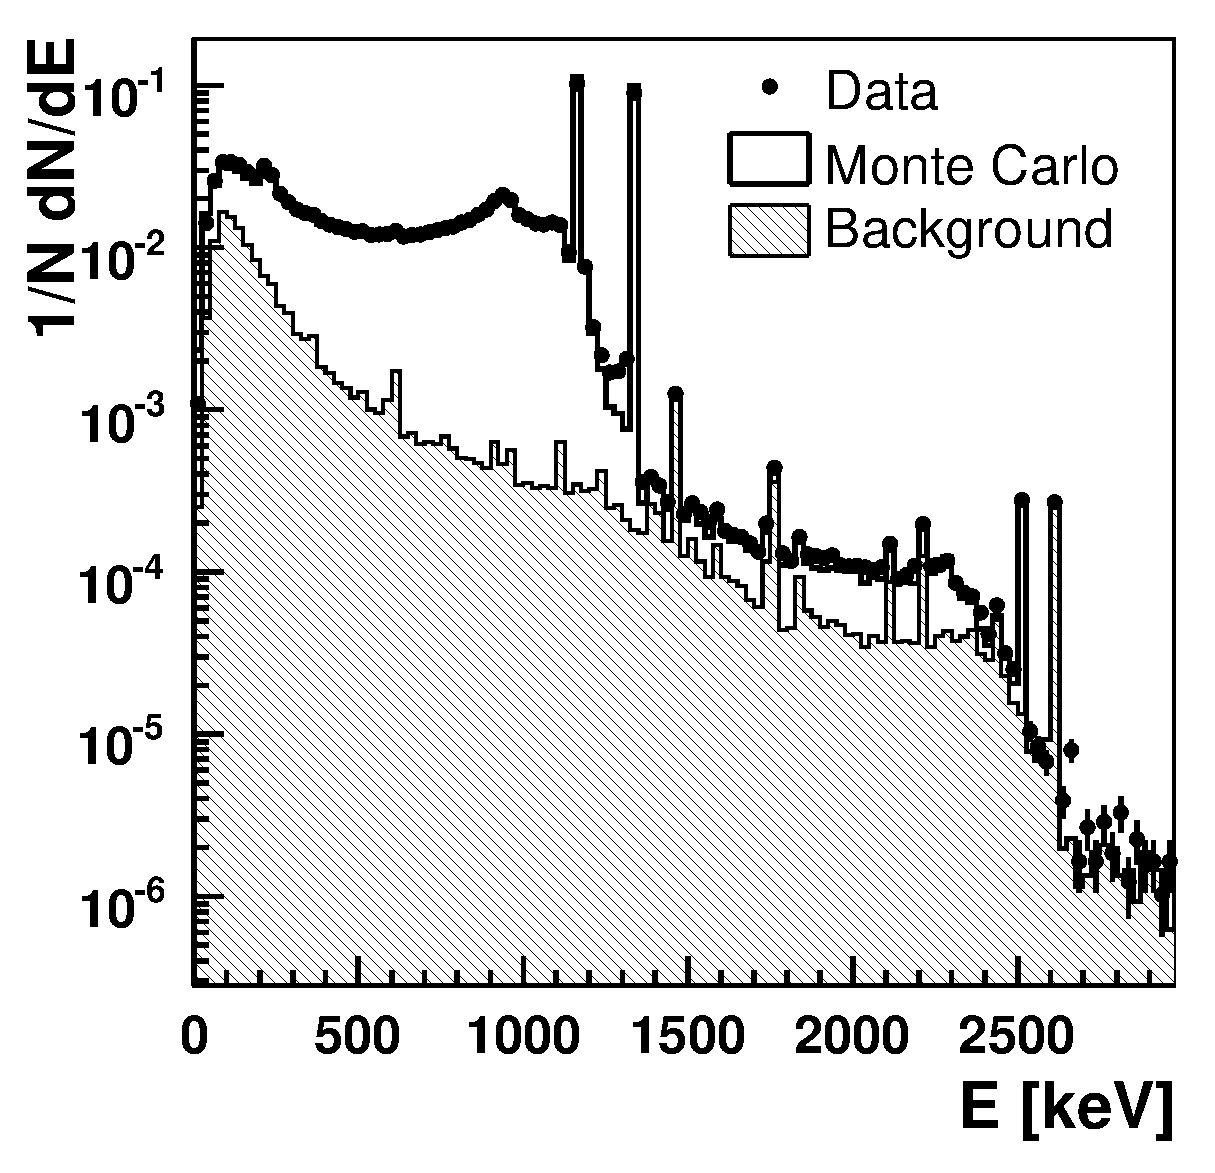
\includegraphics[width=0.45\textwidth]{datatomc_core_energy}}%
\subfloat[Occupancy of all segments]{\label{fig:ph:mcb}
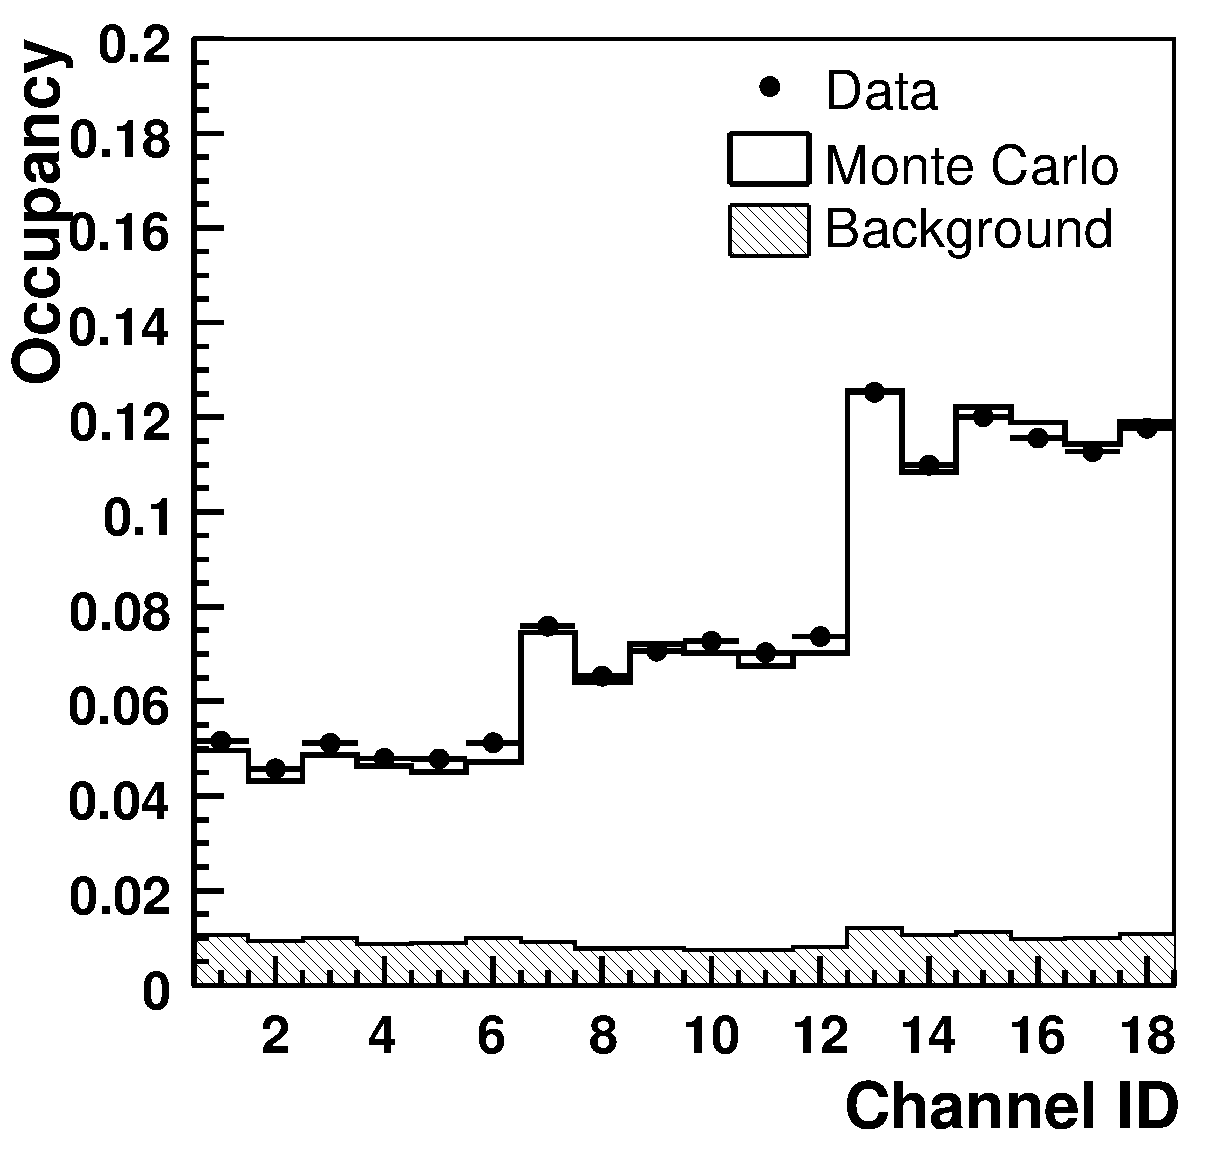
\includegraphics[width=0.45\textwidth]{datatomc_occupancy}}\\
\subfloat[Segment multiplicity]{\label{fig:ph:mcc}
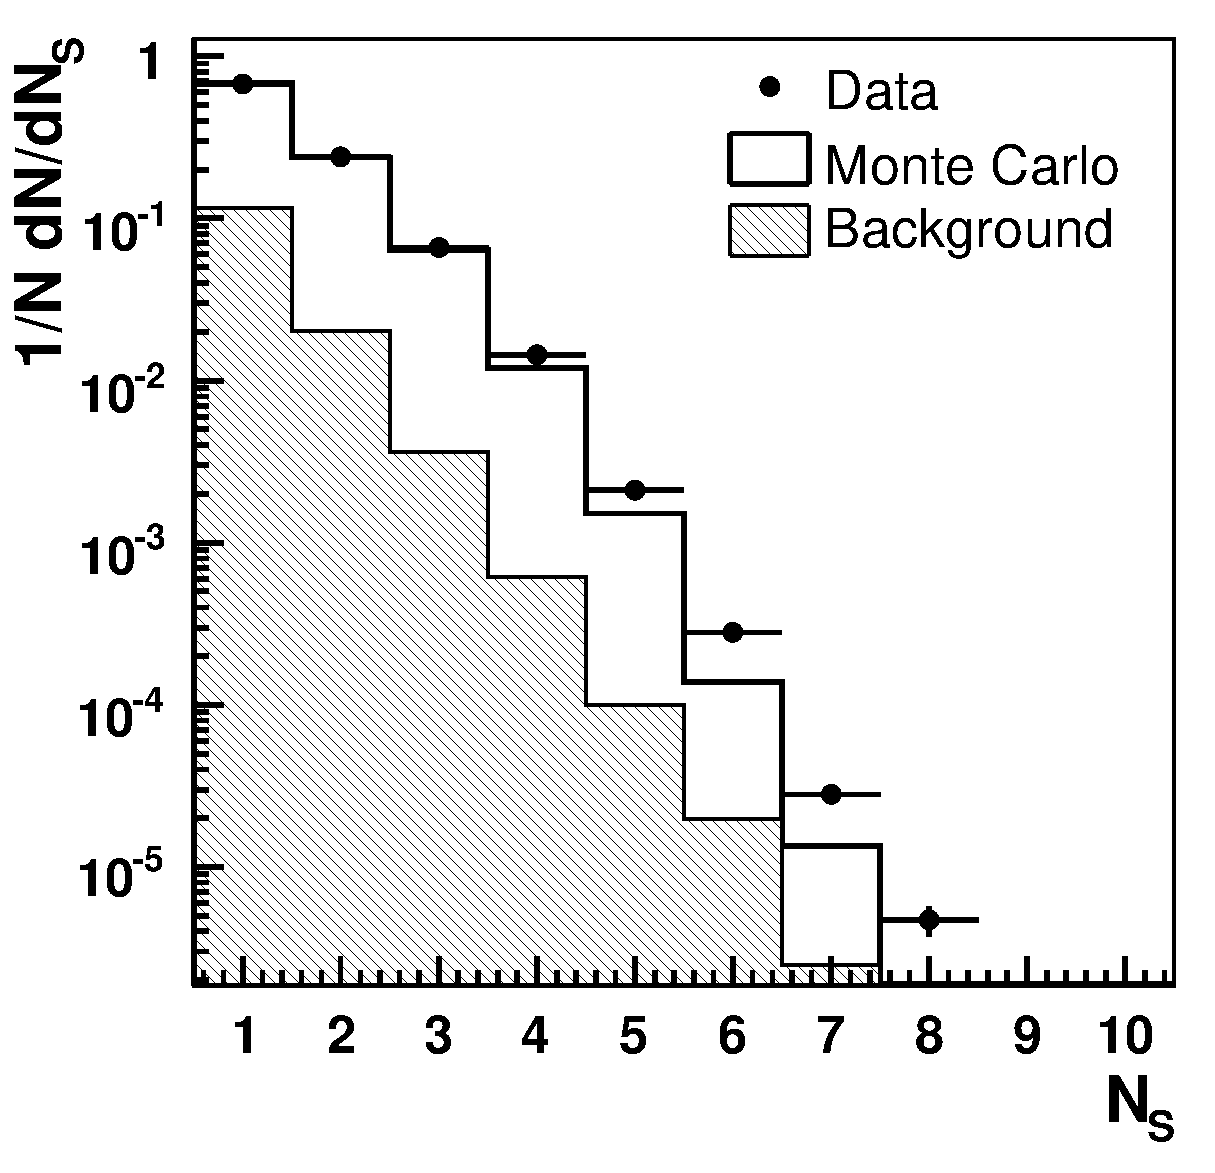
\includegraphics[width=0.45\textwidth]{datatomc_multiplicity}}%
\subfloat[Suppression factors]{\label{fig:ph:mcd}
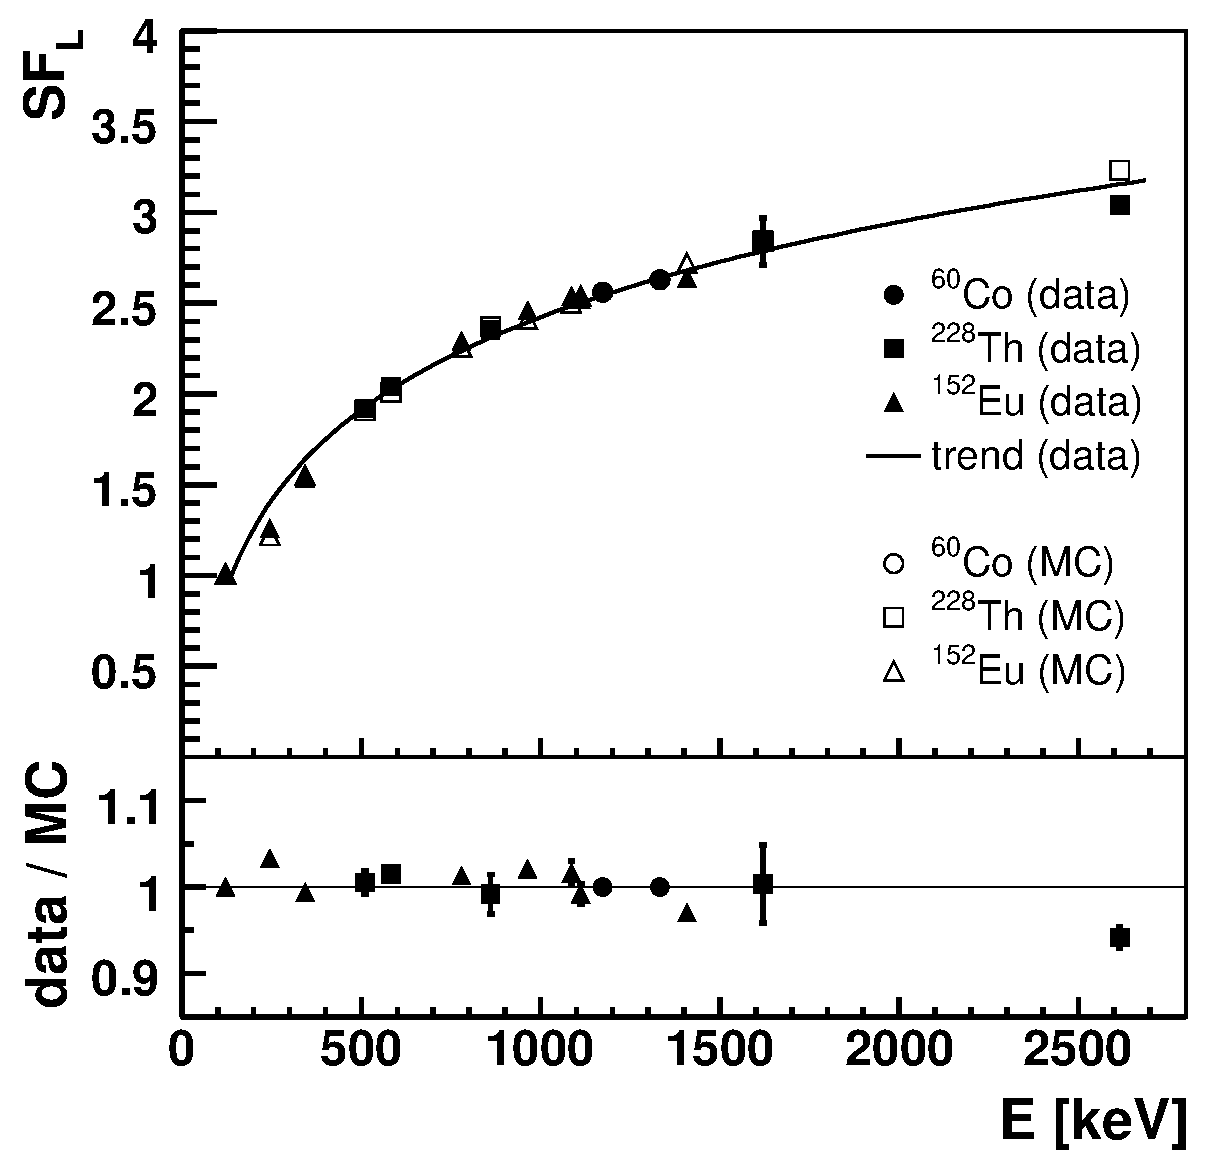
\includegraphics[width=0.45\textwidth]{suppression}}%
\caption{Comparison between data (dots with error bars) and MC (open histogram) plus background (hatched histogram) for several quantities under study. Plots are taken from Ref.\cite{Pid07}}
\label{fig:ph:mc}
\end{figure}

The MC simulation agrees with data very well in general. Some discrepancies are related to the charge carrier drift inside the germanium detector which cannot be simulated using Geant4 and has to be treated in other ways. As shown in Fig.~\ref{fig:ph:mca} the low energy side of the 1332~keV peak in data is significantly higher than that in MC. This is probably due to the surface channel effect as described in Ref\cite{Sur05}. The occupancy distribution as shown in Fig.~\ref{fig:ph:mcb} was measured with the experimental setup shown in Fig.~\ref{fig:ph:occ}. The $\gamma$ source was placed on top of the detector. Naturely, the top layer of the detector (segment Nr. 13 - 18) had the highest event rate, the bottom layer (segment Nr. 1 - 6) had the lowest event rate. The event rates of different segments in the same layer should have been the same because the source were put right on top of the core of the detector (see Fig.~\ref{fig:ph:occ}b). However, this is not the case as shown in Fig.~\ref{fig:ph:mcb}. This is because the drift of charge carriers are affected by the structure of the germanium crystal, the drift trajectories do not follow the electric field lines consiquently. This effect cannot be simulated using Geant4. An effective model was used to tune the simulated distribution in order to minimize the discrepancy betwen MC and data. The full simulation of the drift of the charge carriers in germanium detectors was done as described in Cha.~\ref{cha:pss} and \ref{cha:psa}.

\begin{figure}[htbp]
\centering
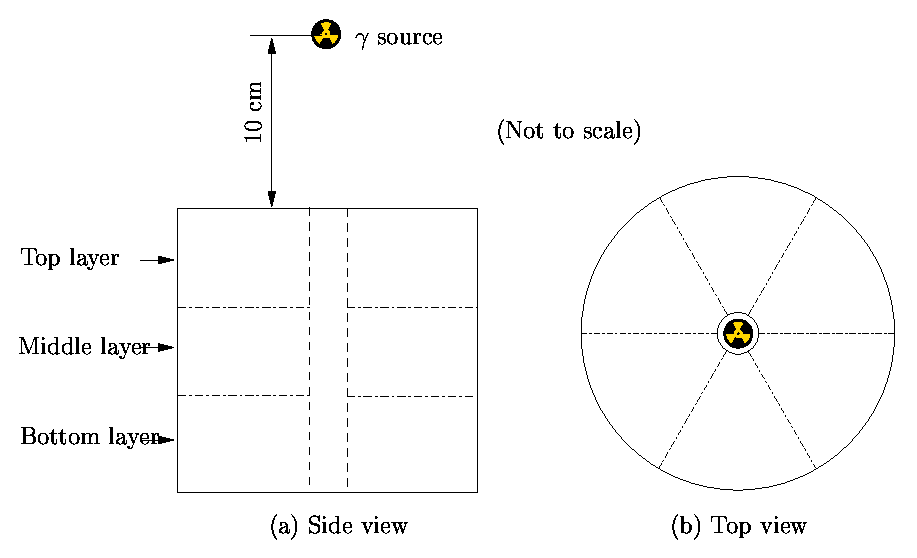
\includegraphics[width=0.8\textwidth]{occumea}
\caption{Schematic of experimental setup for occupancy measurement.}
\label{fig:ph:occ}
\end{figure}

%%% Local Variables:
%%% mode:latex
%%% TeX-master: "thesis"
%%% End: